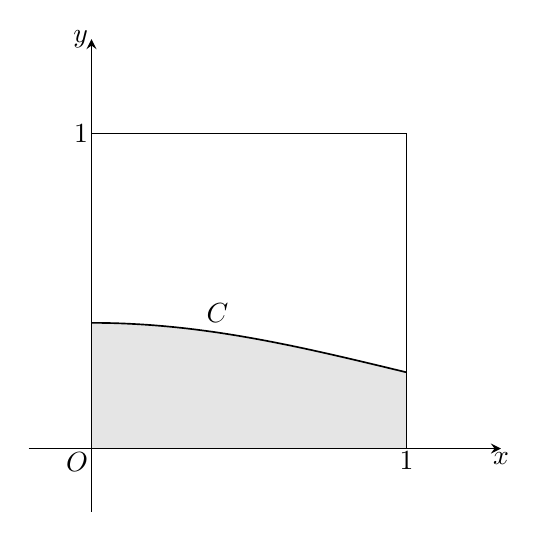
\begin{tikzpicture}[line width=0.6pt, font=\normalsize, >=stealth]
% unit square [0,1]x[0,1], 4cm per unit; curve C = standard normal pdf
\def\s{4}
\coordinate (O) at (0,0);
% shaded region under curve C over [0,1]
\fill[gray!20] (0,0) -- (0,1.5956) --
  plot[domain=0:1, samples=60, smooth] ({\x*\s}, {exp(-\x*\x/2)/2.5066283*\s})
  -- (\s,0) -- cycle;
% square
\draw (0,0) rectangle (\s,\s);
% curve C: phi(x)=exp(-x^2/2)/sqrt(2pi)
\draw plot[domain=0:1, samples=60, smooth] ({\x*\s}, {exp(-\x*\x/2)/2.5066283*\s});
% axes
\draw[->] (-0.8,0) -- (5.2,0);
\draw[->] (0,-0.8) -- (0,5.2);
\node[below left, inner sep=1pt] at (0,0) {$O$};
\node[below, inner sep=1pt] at (5.2,0) {$x$};
\node[left, inner sep=1pt] at (0,5.2) {$y$};
\node[below, inner sep=1pt] at (\s,0) {$1$};
\node[left, inner sep=1pt] at (0,\s) {$1$};
\node[above, inner sep=1pt] at (1.6,1.55) {$C$};
\end{tikzpicture}
